\documentclass[10pt,unicode]{beamer}
\usetheme{ttiposter}

% geometries

\geometry{paper=a4paper,landscape}

% packages

\usepackage{luatexja}
\usepackage{amsmath}

% miscellaneous commands

\newcommand{\columnsize}{0.32}
\newcommand{\tablefontsize}{\small}
\newcommand{\itemtitle}[1]{{\large #1} \\}
\newcommand{\arrow}{{\color{orange} →}\hspace{1ex}}

% title setting

\title{カテゴリ間の関連性を利用した多層ニューラルネットワークによる文書分類}
\author{外山洋太、三輪誠、佐々木裕}
\institute{豊田工業大学 工学部 先端工学基礎学科}
\date{}


\begin{document}
\begin{frame}{}
\maketitle
\begin{columns}[t]

\begin{column}{\columnsize\textwidth} % first
  \begin{block}{背景と目的}
    \begin{itemize}
      \item 文書を複数のカテゴリについて多値分類 \\
      (カテゴリ:ラベルが付けられる各項目のこと)
      \item 従来の手法[1]
        \begin{itemize}
        \item カテゴリ同士の関連性を手動で変化させ考慮 \\
        \arrow 機械学習による自動化
        \item 文書の数値表現であるBoWは文書内の語順を無視 \\
        \arrow パラグラフベクトルの使用により表現をより正確に
        \end{itemize}
    \end{itemize}
  \end{block}

  \begin{block}{\bf 関連研究}
    \begin{itemize}
    \item \itemtitle{カテゴリ間の関連性を用いた文書分類}
    カテゴリ間の関連性を用いた文書分類を扱った研究に、隠れ状態を用いた
    ホテルレビューのレーティング予測[1]がある。この研究では、文書内の各文に対して
    推定した隠れレーティングとレビュー全体のレーティングとの繋がりを変化させ、
    カテゴリ間の関連性を考慮した分類を行っている。
    \item \itemtitle{パラグラフベクトル}
     文書の数値表現の一つとして、Leら[2]が提案したパラグラフベクトルがある。
    この研究は、それが文書分類に有用であることを実験により示している。また、
    パラグラフベクトルの学習手法に関する研究として、森ら[3]がある。この研究では、
    単語同士の位置関係を考慮した単語ベクトルの学習手法vLBL+vLBL(c)について、
    パラグラフベクトルまたは文ベクトルも同時に学習する手法を提案している。
    \end{itemize}
  \end{block}
\end{column} % first

\begin{column}{\columnsize\textwidth} % second
  \begin{block}{提案手法}
     文書の意味を的確に表現するためにvLBL+vLBL(c)の応用手法によって生成した
    パラグラフベクトル及び文ベクトルを、カテゴリ間の関連性を考慮するために
    多層ニューラルネットワーク(NN)による分類器を用いた文書分類を行う。
    まず、パラグラフベクトルに加え文ベクトルを導入したvLBL+vLBL(c)を提案し、
    語順と単語同士の位置関係を考慮した文書の数値表現を生成する(図1)。
    ここで、文ベクトル学習時の目的関数gには以下の式を用いる。

    \begin{eqnarray*}
      g = & \sum_t \left\{ \log\sigma(s(t))
          + \sum^K_{t' \sim P_n} \log(1 - \sigma(s(t'))) \right\} \\
      s(t) = & {\bf c}_t \cdot {\bf w}_t
             + {\bf c}^{loc}_t \cdot {\bf w}^{loc}_t + b_t
    \end{eqnarray*}

    tは現在の単語の位置、ctとwtはそれぞれ文脈と単語を表すベクトル、sは位置関係を
    考慮した単語と文脈の類似度である。上式により、現在の単語は文脈と意味が
    近くなるように、文脈外の単語t'については単語の頻度分布PnについてK回サンプルし
    文脈と意味が遠くなるように学習を行う。また、σはシグモイド関数である。
    次に、多層NNへの入力をパラグラフベクトル、及び、各文ベクトルの
    平均ベクトルとし、出力をカテゴリ毎のラベルとして教師有り学習を行う。
    分類時も同様な処理を行いラベルを推定する。

    \begin{figure}
      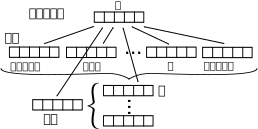
\includegraphics{fig/vectors.png}
      \caption{単語及び文、文章ベクトルの学習}
    \end{figure}
  \end{block}
\end{column} % second

\begin{column}{\columnsize\textwidth} % third
  \begin{block}{予備実験}
    パラグラフベクトルの学習手法としてvLBL+vLBL(c)を、分類器として
    SVMまたは多層NNを用い、従来の手法[1]と同じ多値分類問題の精度を測定

    \begin{itemize}
      \item \itemtitle{目的}
      \begin{itemize}
        \item パラグラフベクトルの有効性の調査
        \item 従来手法との比較による目標設定
      \end{itemize}

      \item \itemtitle{実験設定}
      \begin{itemize}
        \item 入力データは、宿泊予約サイト楽天トラベルにおける各ホテルレビューの
        コメント部分とそのユーザが付けた食事、サービスなど7カテゴリのレーティングの
        組(各カテゴリのレーティングは評価なしを含む6段階評価)
        \item 全レビュー338,028件の内、
        訓練データ:300,000件、評価データ:10,000件
        \item 多層NNの入力は位置を考慮した及び考慮していない2つの
        パラグラフベクトル
      \end{itemize}

      \item \itemtitle{結果及び考察}
      \begin{itemize}
        \item 多層NNを用いた方がSVMより4.1pp精度が高い
        しかし、多層NNを用いた手法でも、従来の手法[1]における精度を10pp以上
        下回っている。精度を高めるためには、文ベクトルとパラグラフベクトルを
        組み合わせより表現力の高い文書の数値表現を評価することや、多層NNの
        パラメータ最適化が必要である。
      \end{itemize}
    \end{itemize}

    \begin{table}
    \tablefontsize
    \caption{点数推定プログラムのパラメータ設定}
    \label{table:parameters}
    \begin{tabular}{l | r}
    項目 & 値 \\
    \hline
    学習する単語の範囲 & 前後5単語 \\
    単語の最少出現回数 & 5回 \\
    ベクトルの次元数 & 400 \\
    中間層の数 & 1 \\
    入力層でのニューロン数 & 800個 \\
    中間層でのニューロン数 & 200個
    \end{tabular}
    \end{table}

    \begin{table}
    \tablefontsize
    \caption{各手法における点数推定精度}
    \begin{tabular}{l | r}
    項目 & 点数推定の精度(\%) \\
    \hline
    実験での手法(SVM)& 33.6 \\
    実験での手法(多層NN)& 37.7 \\
    従来の手法[1] & 48.3
    \end{tabular}
    \end{table}
  \end{block} % 実験

  \begin{block}{今後の課題と改善策}
    \begin{itemize}
    \item 文ベクトルの評価
    \item 多層NNのパラメータ最適化
    \item 提案手法の有用性の評価
    \end{itemize}
  \end{block} % まとめ

  参考文献 \\
  \begin{itemize}
  \item 藤谷宣典ら, 隠れ状態を用いたホテルレビューのレーティング予測.
  言語処理学会 第21回年次大会, 2015. \\
  \item Quoc Le et al., Distributed Representations of Sentences and Documents.
  ICML 2014, 2014. \\
  \item 森洸樹ら, 英文穴埋め問題における文章ベクトルと学習データの質の影響.
  第222回自然言語処理研究会, 2015.
  \end{itemize}
\end{column} % third

\end{columns}
\end{frame}
\end{document}
